\chapter{Benutzeroberfläche}
\label{ch:benutzeroberfläche}

\begin{figure}
	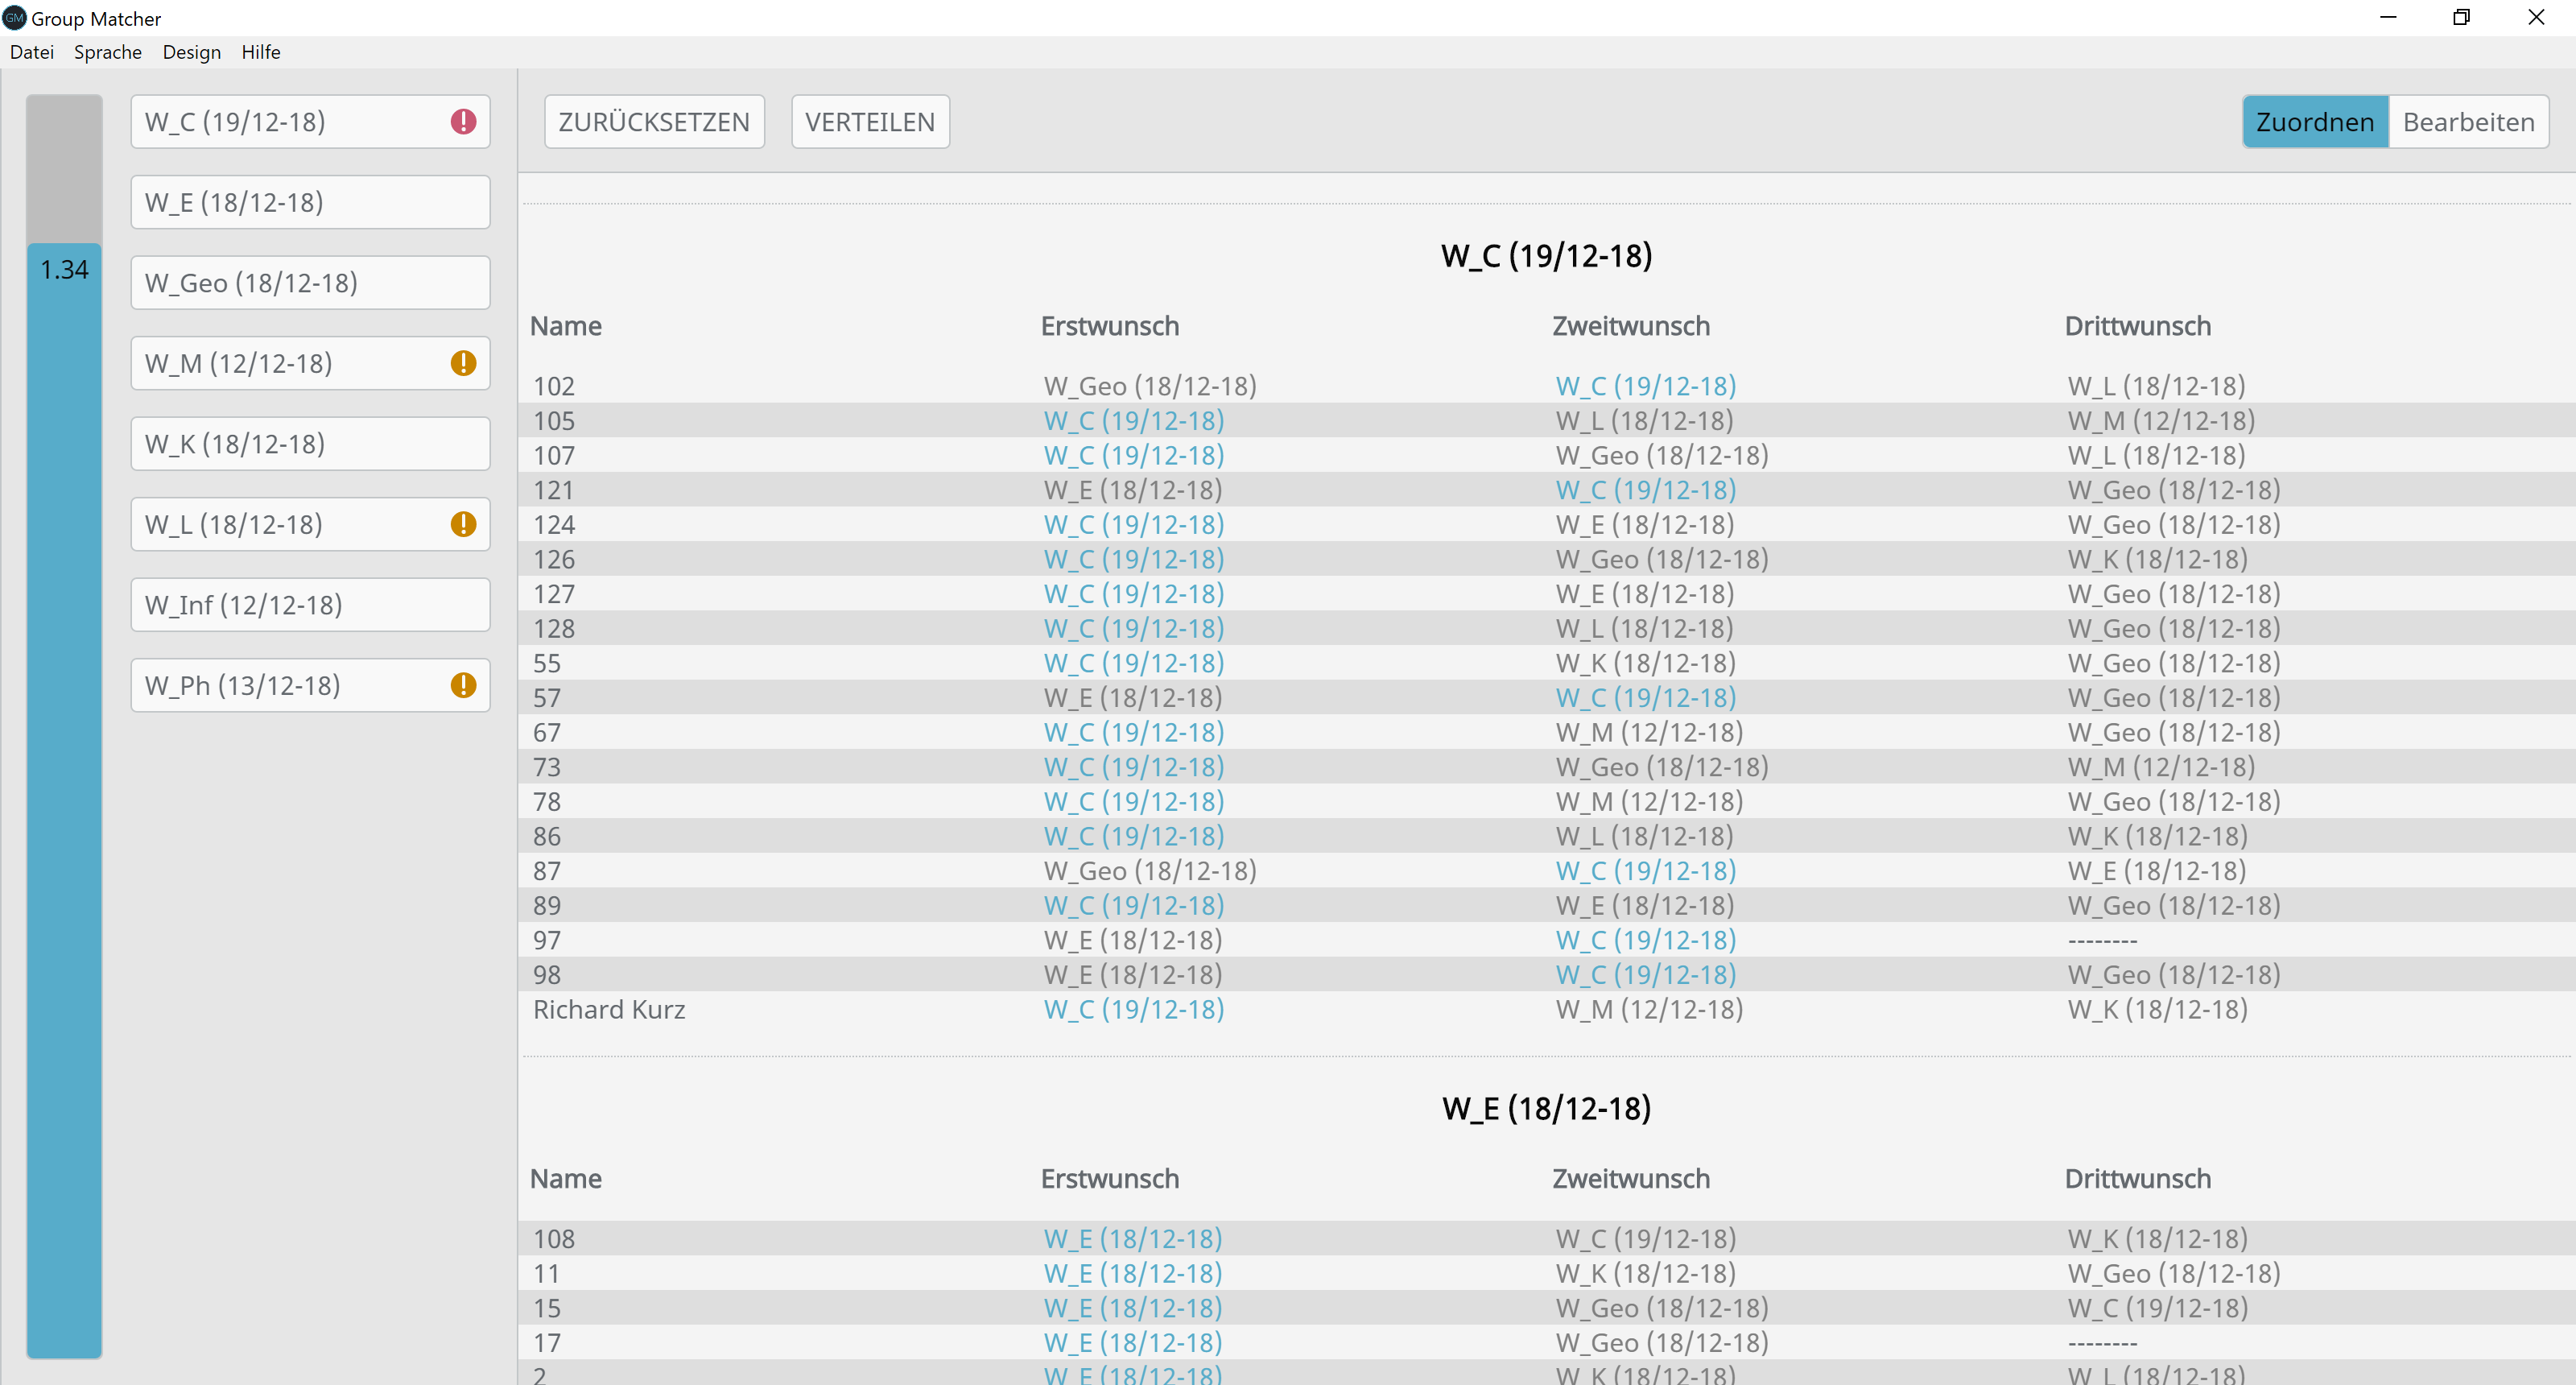
\includegraphics{zuordnungsmodus}
	\caption{Die Benutzeroberfläche}
	\label{fig:die_benutzeroberfläche}
\end{figure}

Die Benutzeroberfläche, die in Abbildung \ref{fig:die_benutzeroberfläche} dargestellt ist, besteht aus vier Bereichen:
\begin{itemize}
	\item Die \hl{Menüleiste}(\ref{sec:menüleiste}) befindet sich in voller Breite ganz oben im Fenster.
	\item Die \hl{Seitenleiste}(\ref{sec:seitenleiste}) nimmt den linken Rand des Bildschirms ein.
	\item Die \hl{Bedienzeile}(\ref{sec:bedienzeile}) ist links von der Seitenleiste und oben von der Menüleiste begrenzt.
	\item Die \hl{Arbeitsfläche}(\ref{sec:arbeitsfläche}) nimmt den Rest des Fensters ein.
\end{itemize}
Die Bedienelemente und deren Nutzen wird im Folgenden erläutert.

\section{Menüleiste}
\label{sec:menüleiste}

Die Menüleiste dient zur Kontrolle von Programm und Projekt. Sie enthält vier Unterpunkte.

\paragraph{Datei} Hier ist zunächst die Kontrolle des Projekts, also der >>.gm<< Datei \mnote{Im Dateiformat >>.gm<< speichert der >>GroupMatcher<< zum einen die Projekte ab. Zum anderen dient das Format auch zur schnellen Erstellung eines Projekts. Die Syntax dafür wird in Kapitel \ref{TODO: label einfügen} beschrieben.} möglich.
\begin{itemize}
	\item \hl{Öffnen...} (öffnet einen Dialog, der das einlesen eines Projekts, also einer >>.gm<< Datei ermöglicht)
	\item \hl{Schließen} (schließt das Projekt, ohne den aktuellen Zustand zu speichern)
	\item \hl{Speichern} (speichert den aktuellen Stand in die geöffnete >>.gm<< Datei)
	\item \hl{Speichern unter...} (öffnet einen Dialog, der das Speichern des aktuellen Standes in eine neue >>.gm<< Datei ermöglicht, und schließt (sofern vorhanden) die alte >>.gm<< Datei)
	\item \hl{Exportieren...} (öffnet einen Dialog, der das erstellen einer Excel-Datei, welche das Projekt darstellt, ermöglicht)
	\paragraph{Excel (begrenzt)} Die begrenzte Version enthält lediglich die Liste der Personen in alphabetischer Reihenfolge mit dem jeweils zugeordneten Wunsch.
	\paragraph{Excel (komplett)} Die komplette Version gibt alle Projektinformationen wieder. Sie listet alle Gruppen mit minimaler und maximaler Mitgliederzahl, sowie der nach der Zuteilung tatsächlich entstandenen Gruppenstärke auf. Zudem stellt sie jede Person mit ihren Wünschen dar und hebt dabei den ihr zugeteilten farblich hervor.
	\item \hl{Beenden} (schließt das Programm und speichert, insofern schon eine >>.gm<< Datei erstellt wurde, das Projekt in diese ab)
\end{itemize}

\paragraph{Sprache} Dieses Untermenü ermöglicht das Wechseln zwischen den bereitgestellten Sprachen.

\paragraph{Design} Neben den hellen Standarddesign lässt sich bei dunkler Umgebung auf das für die Augen angenehmere dunkle Design umschalten.

\paragraph{Hilfe} Neben dem öffnen dieser Dokumentation im Punkt >>Hilfe<< können hier im Punkt >>Über GroupMatcher<< weitere Informationen über Ursprung, aktuelle Versionen und Lizensierung des Programms gewonnen werden.

\section{Seitenleiste}
\label{sec:seitenleiste}

Die Seitenleiste gibt eine Übersicht über das Projekt und erleichtert die Navigation in der Arbeitsfläche. Die blaue Skala zeigt die aktuelle Quote \mnote{Die Quote gibt an, wie zufrieden die Personen durchschnittlich mit ihrer Zuteilung sind. Die genaue Berechnung wird in Abschnitt \ref{TODO:referenz einfügen} genauer erläutert. Generell gilt aber, je höher der blaue Balken, desto besser das Ergebnis.}.\\
Rechts daneben sind alle Gruppen aufgelistet. Dabei wird erst der Gruppenname und dann in Klammern zunächst die aktuelle Gruppenstärke, dann die Mindest- und Maximalgröße der Gruppe angezeigt. Drückt man auf den Knopf einer Gruppe, so scrollt die Arbeitsfläche zu deren Position. Die Knöpfe können zwei verschiedene Warnungen anzeigen. Erscheint ein orangenes Ausrufezeichen, dann bedeutet dies, dass die Gruppe ein Mitglied hat, das unzufrieden \mnote{Unzufriedenheit bedeutet dabei, dass der Person ein Wunsch zugeordnet wurde, der in der hinteren Hälfte seiner Wunschliste steht.} mit seiner Zuteilung ist. Leuchtet stattdessen ein rotes Ausrufezeichen auf, so widerspricht die aktuelle Gruppenstärke der Mindest- oder Maximalgröße der Gruppe. Dieser Fall tritt jedoch nie durch die automatische Verteilung auf, sondern kann nur in der manuellen Nachverteilung herbeigeführt werden. Mehr zum Verteilungsvorgang finden sie in Kapitel \ref{ch:verteilen_der_personen}.
